\documentclass[a4paper,12pt]{article}
\usepackage[utf8]{inputenc}
\usepackage[french]{babel}
\usepackage[T1]{fontenc}
\usepackage[top=2cm,bottom=2cm,left=2cm,right=2cm]{geometry}
\usepackage{graphicx}
\usepackage{wrapfig}
\usepackage{url}

\begin{document}

\begin{titlepage}
	\begin{center}
		\Large{Année universitaire 2016-2017}\\
		\Large{Université de Caen Basse-Normandie}\\[1cm]
		
		\huge{Rapport sur la mise en place de l'XML avec Python dans notre IDE}\\
		\vspace{3cm}
		
		Alexis Carreau
		
	\normalsize{\textit{ ~ L2 Informatique}}\\
		\medskip
		\vspace{2cm}
		
	\begin{figure}[h!]
			\begin{center}
				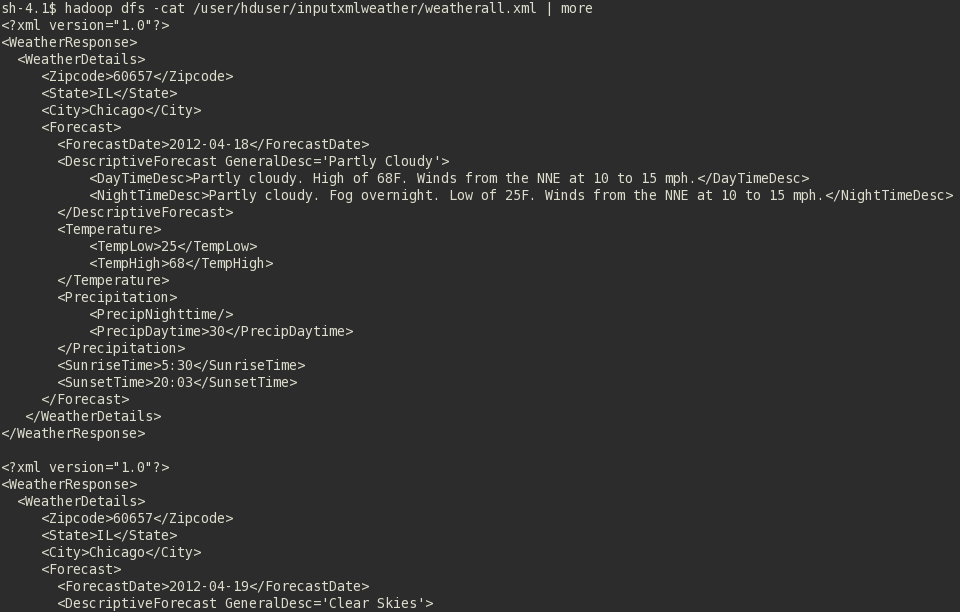
\includegraphics[scale=0.7]{images/intro.png}
				\caption{Exemple de fichier XML}
			\end{center}
		\end{figure}
				
	\end{center}
\end{titlepage}

\tableofcontents
\newpage

\section{La nécessité du XML}

Au fur et à mesure de l'ajout de fonctionnalités dans notre IDE, l'utilisation du XML s'est vite imposée du fait de son efficacité et également par convention. Nous devions ainsi lire, parcourir et écrire dans un fichier XML afin de subvenir à nos besoins dans l'élaboration des différentes fonctionnalités de notre IDE dans différentes conditions. Nous utilisons plusieurs fichiers xml, un pour chaque projet, un pour tous les projets et un fichier de configuration.
	
\section{XML et Python : LXML}

Pour ce faire, nous avons utilisé LXML, qui nous permet d'utiliser des outils de parse XML dans notre IDE avec Python. En effet, l'outil "etree", après son import, nous permet de parser un fichier XML et de le parcourir et modifier par la suite.
		
Nous avons beaucoup d'outils disponibles pour parcourir et modifier un fichier XML : 

\begin{figure}[h!]
			\begin{center}
				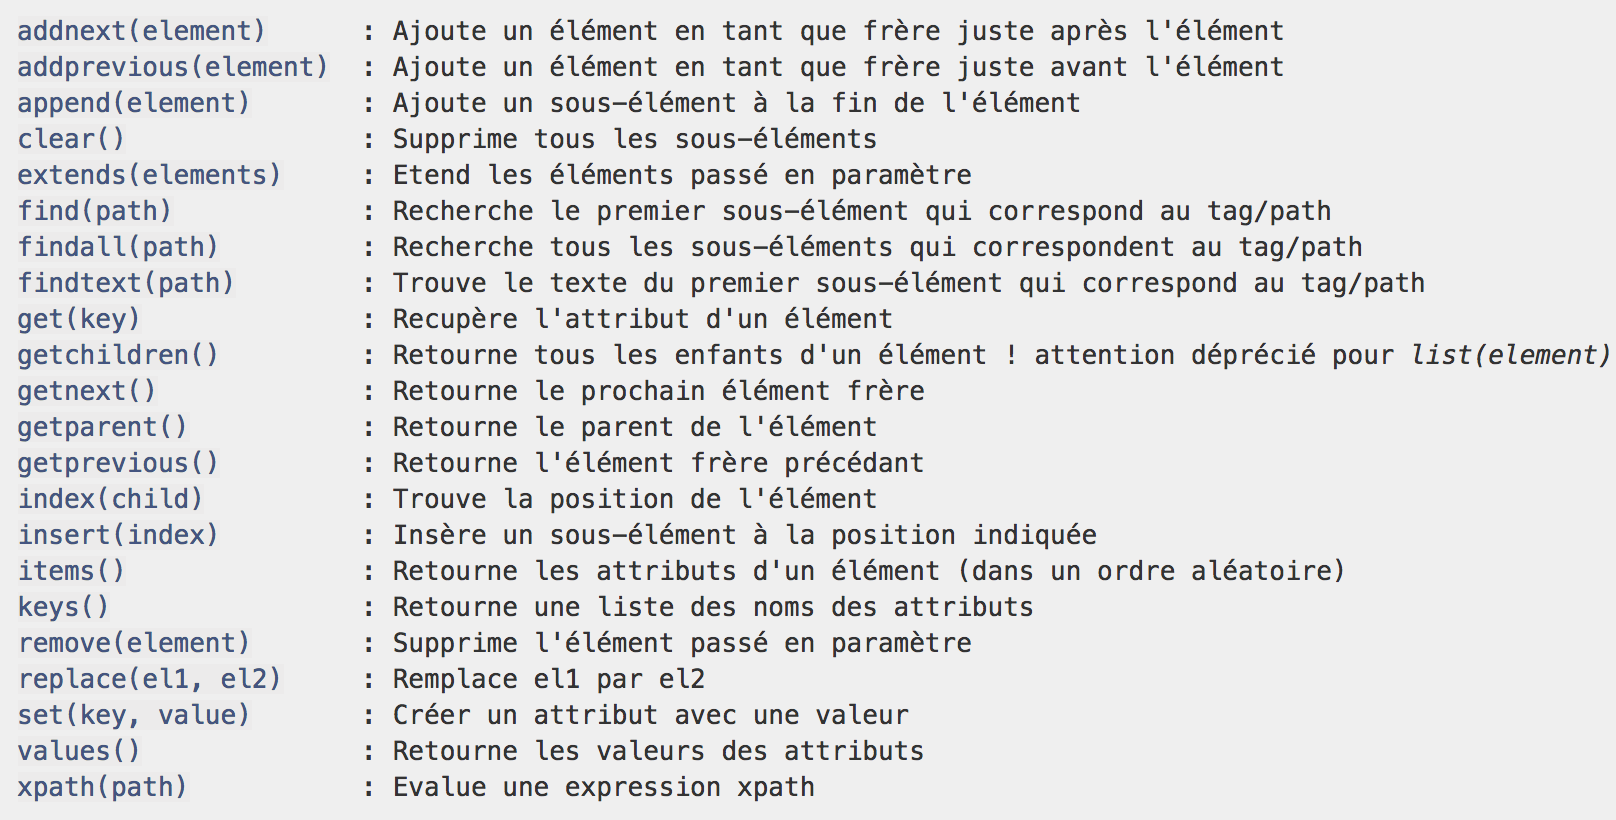
\includegraphics[scale=0.6]{images/lxml.png}
				\caption{Outils LXML disponibles}
			\end{center}
		\end{figure}

Nous avions donc ainsi tous les outils nécessaires pour utiliser le XML dans notre IDE. Nous avons d'ailleurs utilisé les outils "find", "getchildren" et "xpath" par exemple pour le parcours du fichier XML.

\section{Le module XML et le fichier de configuration}

Nous avons donc ainsi créer un module XML pour les fonctions de parcours et d'écriture de fichier XML et bien entendu, le fichier de configuration XML. Voici d'ailleurs leur disposition dans notre IDE, ils sont à la racine du projet.

\newpage

\begin{figure}[h!]
			\begin{center}
				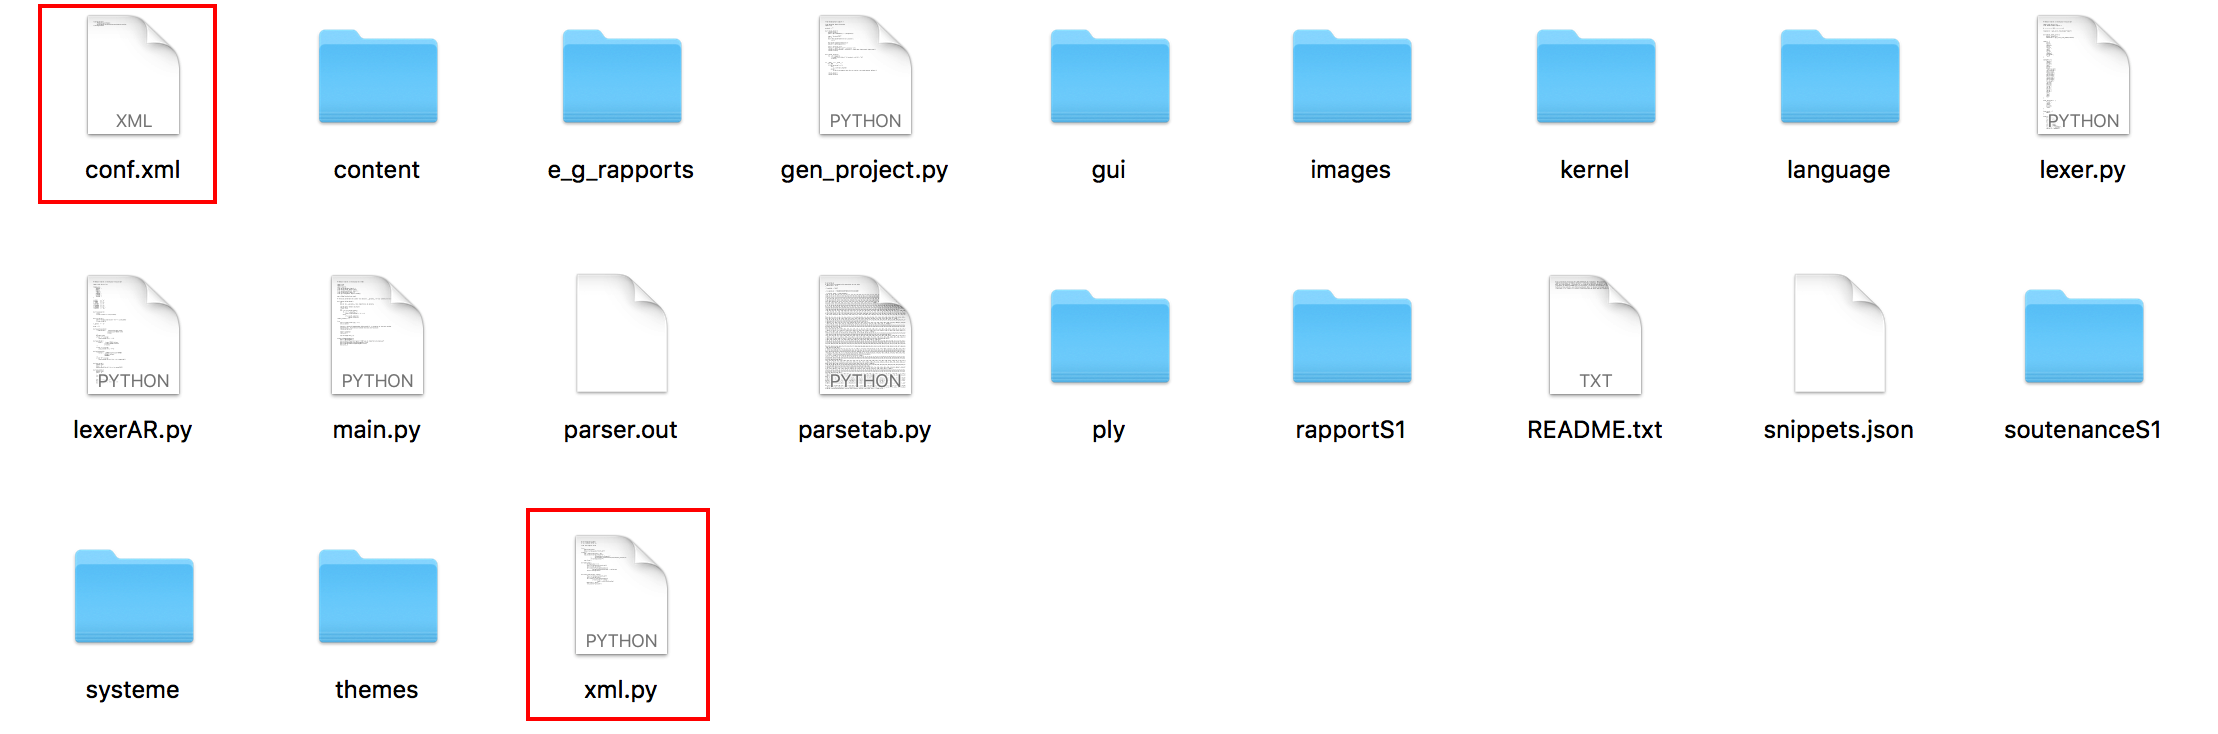
\includegraphics[scale=0.23]{images/dossier.png}
				\caption{Disposition du module et du fichier de configuration}
			\end{center}
		\end{figure}
		
Dans le module XML, nous avons une fonction open\_xml, qui ouvre, parse et parcours le fichier de configuration XML pour retourner un dictionnaire avec comme clés le nom des balises XML, et comme valeurs la valeur des balises. Nous avons également une fonction write\_xml qui permet d'écrire des modifications dans le fichier de configuration. On rentre le nom d'une balise et la valeur voulue en arguments, la fonction trouve la balise et lui associe cette valeur, puis nous écrivons dans le fichier. Enfin, pour éviter tout problème, si le fichier de configuration n'existe pas ainsi que le fichier comportant tous les projets, on les créé et leur ajoute les valeurs de configuration de base. 
		
Dans le fichier de configuration XML, nous utilisons une balise pour stocker, le thème sélectionné actuellement, le booléen suivant l'activation ou non de l'assistance vocale dans l'interface graphique, le booléen suivant l'activation ou non de l'écran de chargement au démarrage, celui de la numérotation des lignes, le langage de l'IDE (Français ou Anglais) ainsi que la localisation du workplace.
		
\begin{figure}[h!]
			\begin{center}
				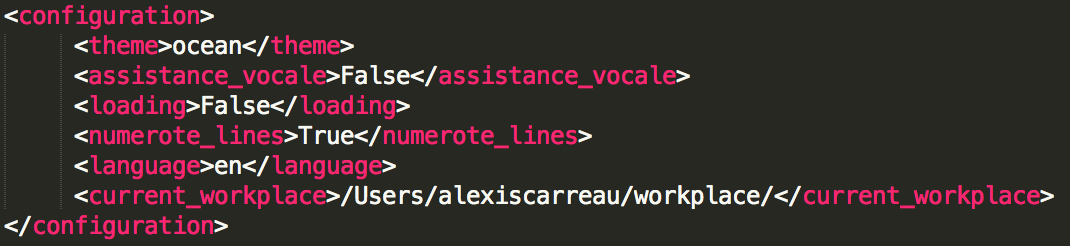
\includegraphics[scale=0.6]{images/conf.png}
				\caption{Fichier de configuration}
			\end{center}
		\end{figure}

\section{L'application dans notre IDE}

Après avoir défini les différentes fonctions et stockage de variables nécessaires, il ne restait plus qu'à implémenter le XML dans notre IDE. Nous l'avons implémentés pour différentes fonctions et nous allons voir des exemples concrets de leur application.

\subsection{Les thèmes}

Pour implémenter le XML pour les thèmes nous devions donc adapter les différentes fonctions déjà définies. Nous l'avons donc fait dans le module thèmes.

Grâce au dictionnaire, nous pouvons ainsi récupérer la valeur du thème actuel en écrivant configuration['theme']. Pour modifier le thème, nous utilisons la fonction write\_xml afin d'associer la valeur en argument à la valeur de la balise theme dans le fichier XML. 

Nous pouvons voir que la mise à jour du fichier XML s'effectue bien suivant le thème sélectionné du fait de sa mémorisation à l'ouverture et fermeture de l'IDE, voilà l'interface graphique de la sélection du thème : 

\begin{figure}[h!]
			\begin{center}
				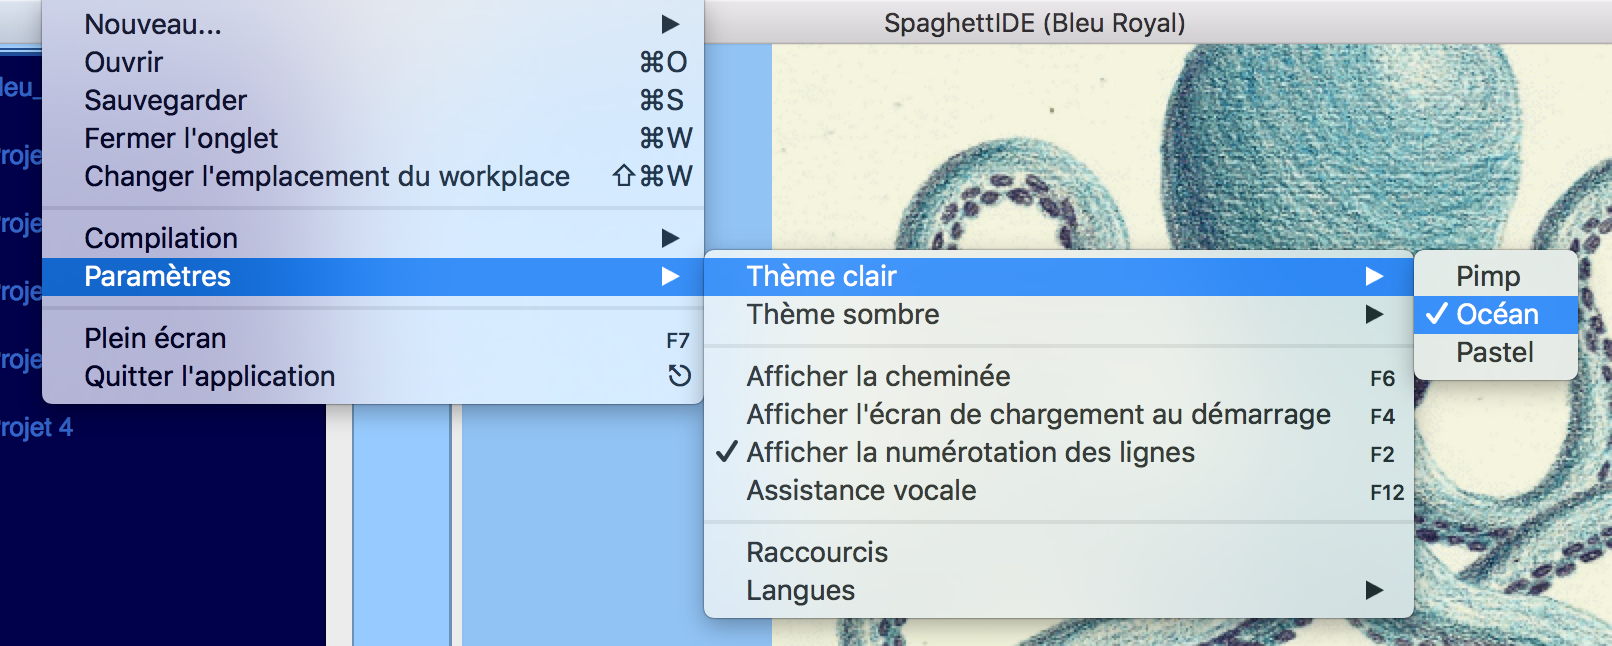
\includegraphics[scale=0.5]{images/themes_selection.png}
				\caption{Interface graphique de la sélection du thème}
			\end{center}
		\end{figure}

\subsection{L'assistance vocale}

L'assistance vocale lit seulement les messages affichés dans la barre de statut et permet ainsi de les dire à voix haute en utilisant la fonctionnalité say de MAC OSX. Donc en fait, on récupère le message de la barre de statut et on le fait dire à voix haute avec cette commande : "os.system("say message")" et le message est renouvelé à chaque clic (si l'assistance vocale est activée bien sûr) sur par exemple l'apparence de l'IDE, donc en cliquant sur un thème dans la barre de menu. Pour implémenter le XML pour l'assistance vocale nous devions donc encore une fois adapter les différentes fonctions déjà définies. Nous l'avons donc d'abord fait dans le module GUI. 

Grâce au dictionnaire, nous pouvons ainsi récupérer la valeur de l'activation de l'assistance vocale actuelle en écrivant configuration['assistance\_vocale']. Nous pouvons ainsi faire des conditions. Nous utilisons encore une fois la fonction write\_xml afin d'associer la valeur en argument à la valeur de la balise assistance\_vocale dans le fichier XML. 

Nous avons adapté les différentes fonctions déjà définies dans le module MENU. Avec encore une fois des conditions, nous avons fait en sorte que si l'assistance vocale était désactivée alors elle n'est pas cochée dans le menu fichier et inversement.

Nous pouvons voir que la mise à jour du fichier XML s'effectue bien suivant l'activation ou la désactivation de l'assistance vocale du fait de sa mémorisation à l'ouverture et fermeture de l'IDE, voilà l'interface graphique de la sélection de l'assistance vocale : 

\newpage

\begin{figure}[h!]
			\begin{center}
				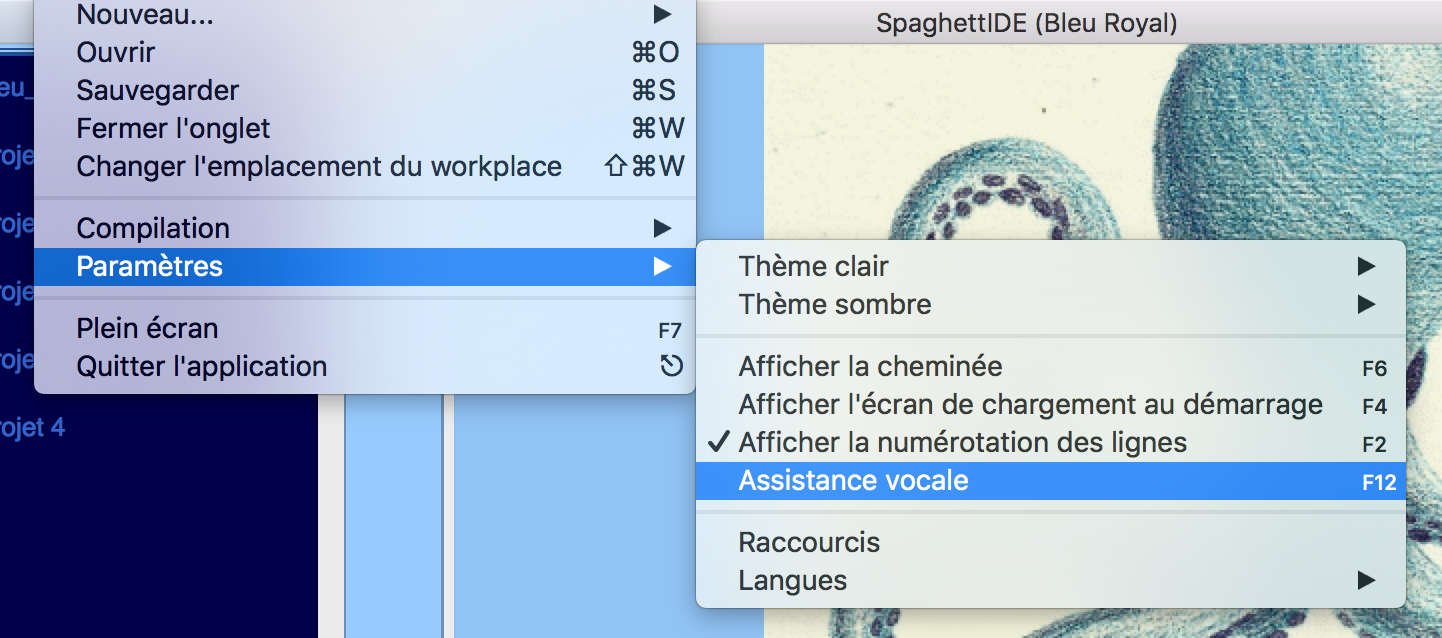
\includegraphics[scale=0.5]{images/assistance_vocale.png}
				\caption{Interface graphique de la sélection de l'assistance vocale}
			\end{center}
		\end{figure}
		
L'assistance vocale n'est disponible pour le moment que sous MAC OSX.
		
\subsection{L'écran de chargement au démarrage}

L'écran de chargement au démarrage est sélectionnable via le menu et il sera ainsi affiché à chaque démarrage de l'IDE en premier plan. Pour ce faire, c'est le même principe que précédemment avec le booléan stocké dans le fichier de configuration xml qui est lu à chaque démarrage de l'IDE. 

\begin{figure}[h!]
			\begin{center}
				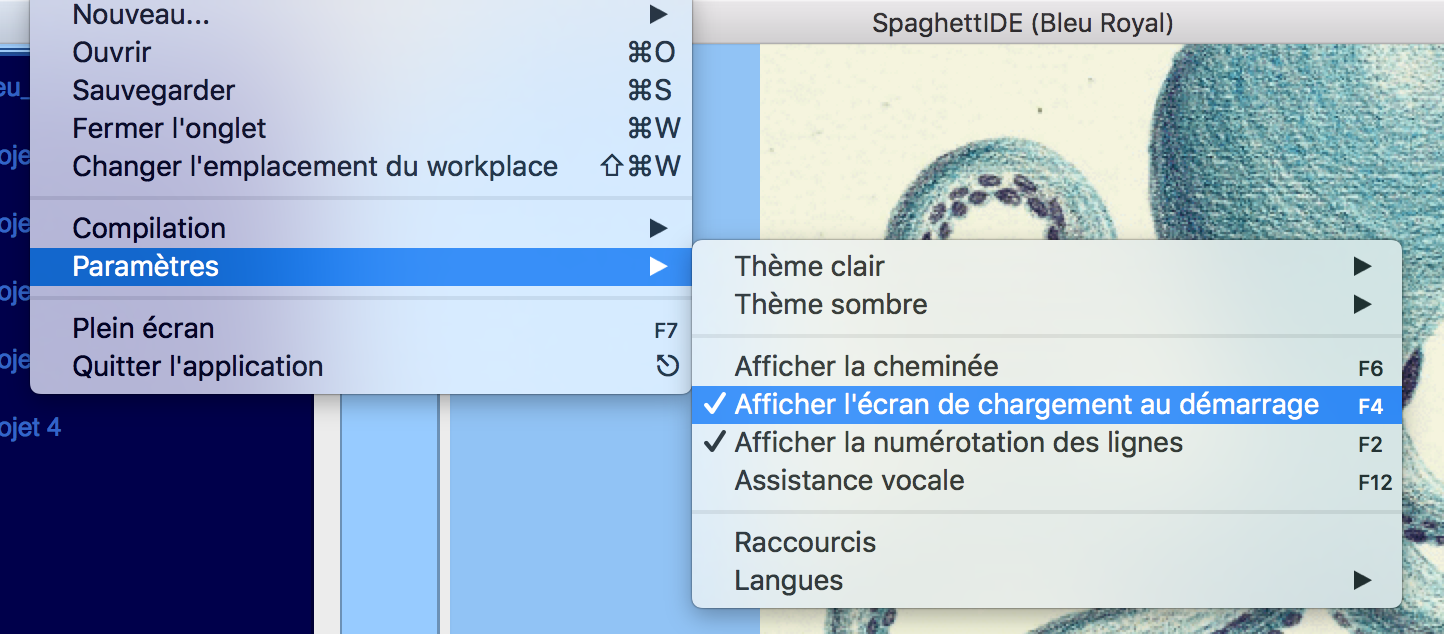
\includegraphics[scale=0.6]{images/selection_loading.png}
				\caption{Interface graphique de la sélection de l'écran de chargement au démarrage}
			\end{center}
		\end{figure}
		
\newpage

\begin{figure}[h!]
			\begin{center}
				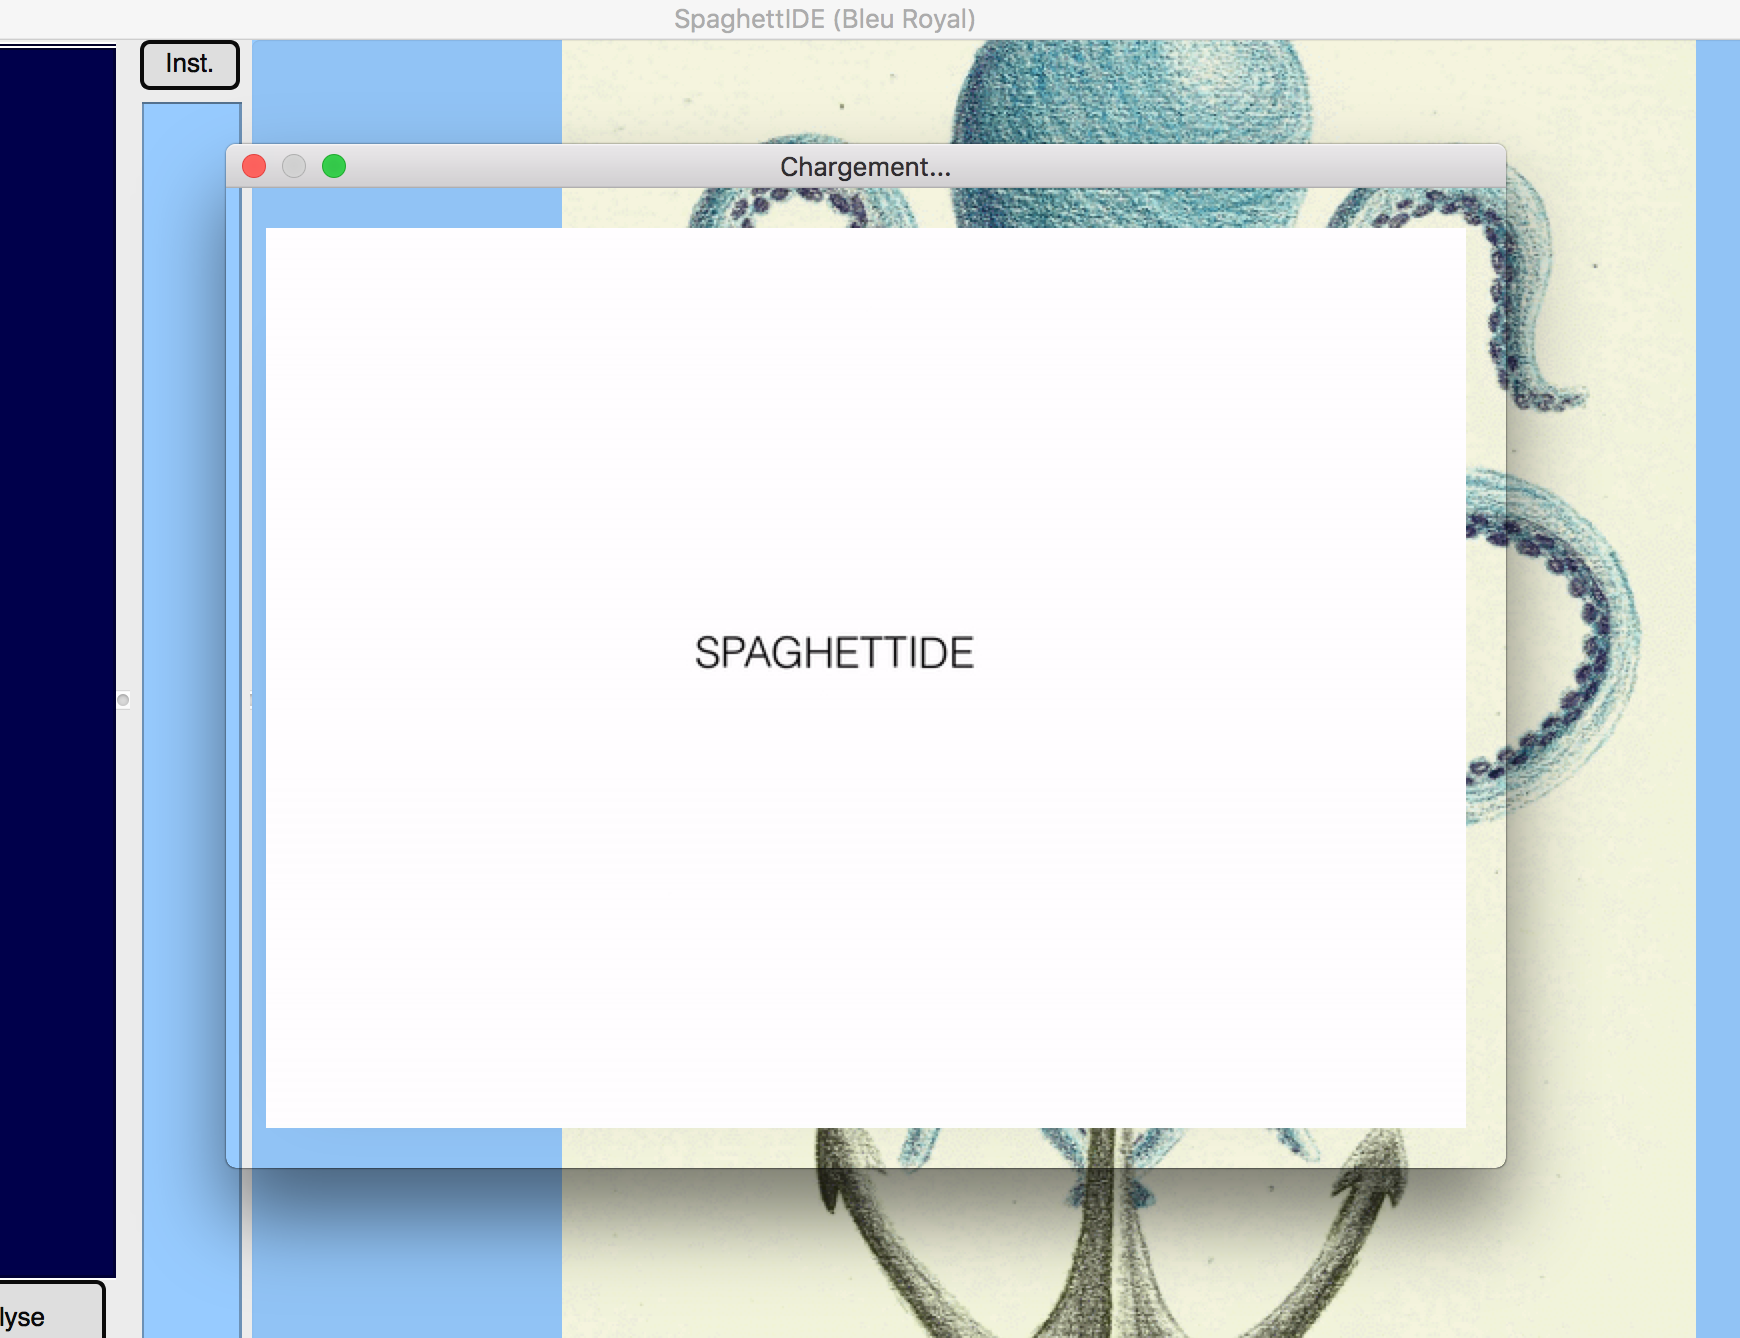
\includegraphics[scale=0.5]{images/loading.png}
				\caption{Écran de chargement au démarrage}
			\end{center}
		\end{figure}
		
\subsection{La numérotation des lignes}

La numérotation des lignes est également sélectionnable via le menu et elle reste tout le temps active après son activation et se complète progressivement après l'ouverture et l'écriture d'un fichier.

\begin{figure}[h!]
			\begin{center}
				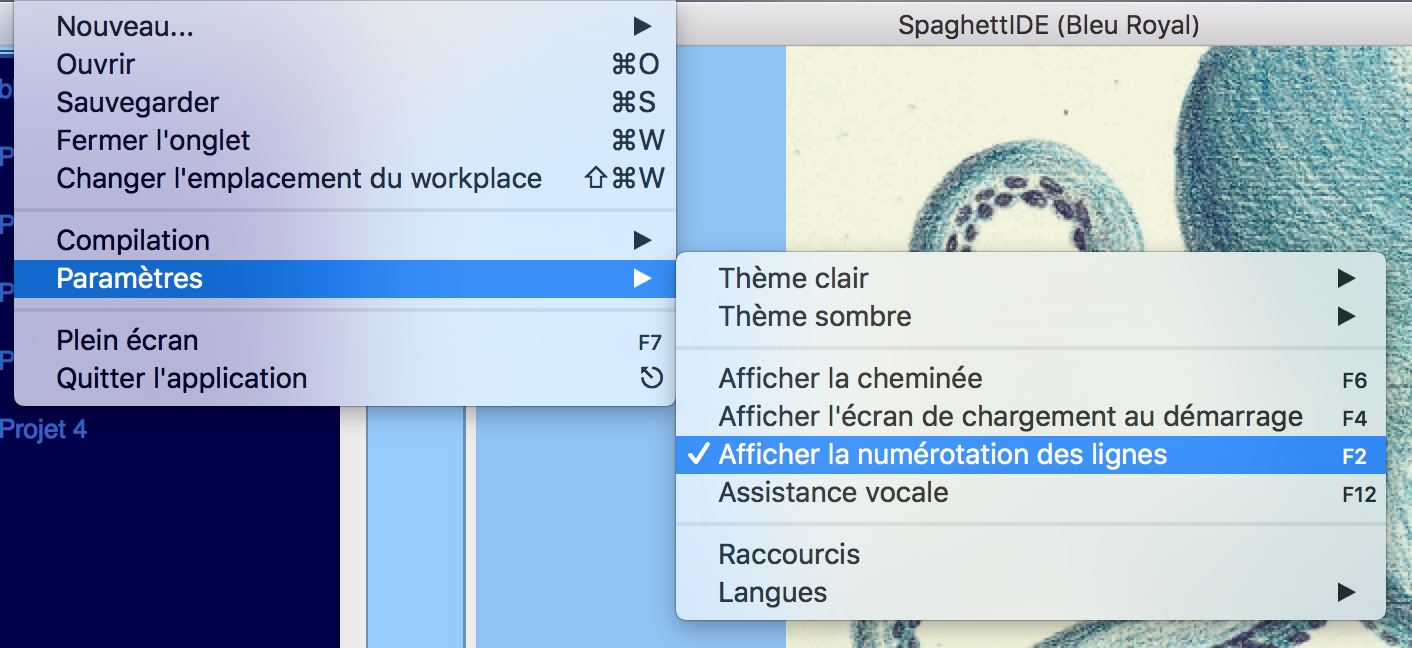
\includegraphics[scale=0.5]{images/selection_numerote_lines.png}
				\caption{Interface graphique de la sélection de la numérotation des lignes}
			\end{center}
		\end{figure}
		
\begin{figure}[h!]
			\begin{center}
				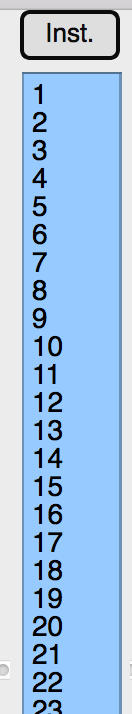
\includegraphics[scale=0.6]{images/numerote_lines.png}
				\caption{Numérotation des lignes}
			\end{center}
		\end{figure}
		
\section{Exemples concrets de l’utilisation du xml dans notre IDE}

Nous allons voir dans cette partie des exemples concrets de l'utilisation des fonctionnalités dans l'IDE. Nous pouvons voir dans l'image ci-dessous la fonction permettant l'activation ou la désactivation de l'assistance vocale. Nous pouvons constater l'utilisation du dictionnaire stockant la valeur de la balise "assistance\_vocale" afin d'écrire la valeur voulue pour son utilisation.

\begin{figure}[h!]
			\begin{center}
				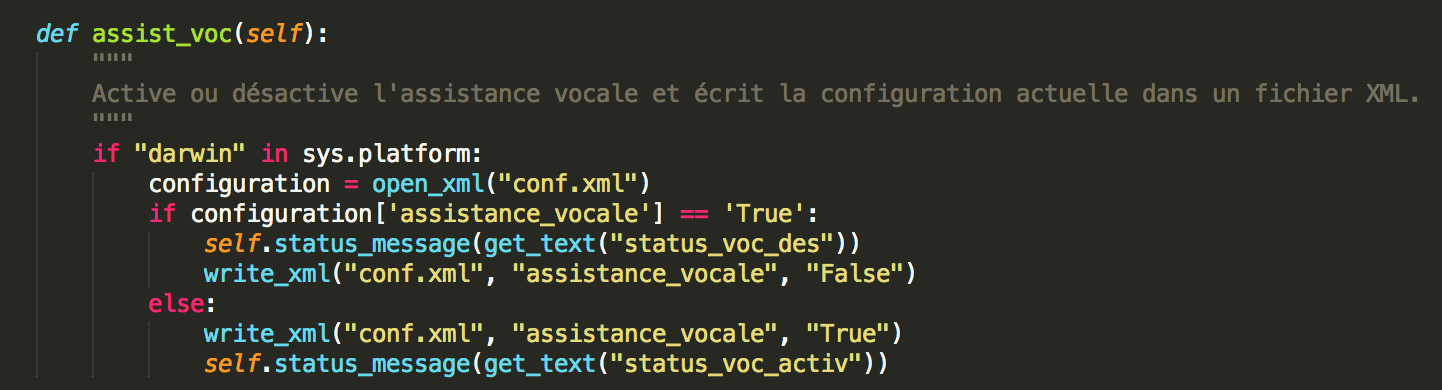
\includegraphics[scale=0.6]{images/assistance_vocale_code.png}
				\caption{Exemple de l'assistance vocale}
			\end{center}
		\end{figure}
		
Nous pouvons voir dans l'image ci-dessous la fonction permettant l'activation ou la désactivation de la numérotation des lignes. Nous pouvons constater encore une fois l'utilisation du dictionnaire stockant la valeur de la balise "numerote\_lines" afin d'écrire la valeur voulue pour son utilisation.

\begin{figure}[h!]
			\begin{center}
				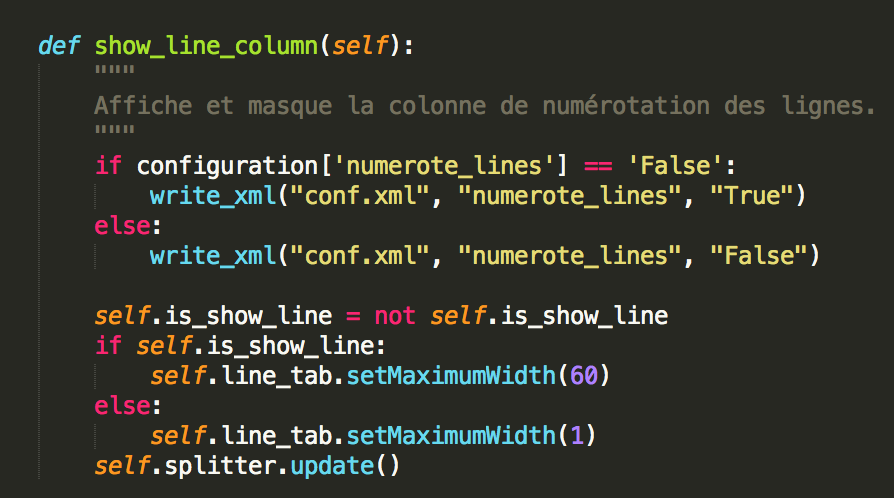
\includegraphics[scale=0.6]{images/numerote_lines_code.png}
				\caption{Exemple de la numérotation des lignes}
			\end{center}
		\end{figure}
	
\section{Les projets et le xml}

Nous allons voir dans cette partie l'utilisation du xml avec les projets. Encore une fois, nous utilisons le dictionnaire stockant les différentes balises et leurs valeurs grâce à la fonction qui parcours un fichier xml et stocke ses données "open\_xml". Dans l'image ci-dessous, nous pouvons voir par exemple l'utilisation de project["name"] pour récupérer le nom du projet, de même avec le langage, la localisation, la date de création et le nombre de fichiers.

\begin{figure}[h!]
			\begin{center}
				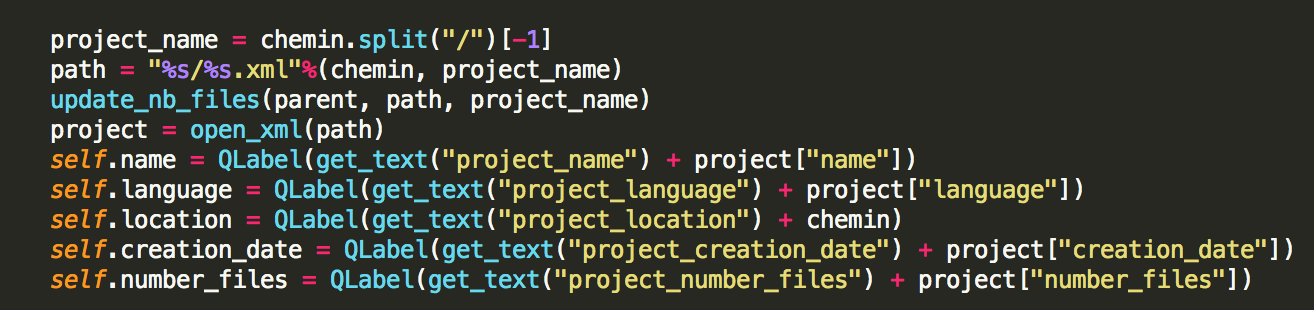
\includegraphics[scale=0.6]{images/projet.png}
				\caption{L'utilisation du xml dans les projets}
			\end{center}
		\end{figure}
		
Voici l'aperçu d'un fichier xml d'un projet avec les différentes valeurs associées aux balises stockées dans ce dernier :

\begin{figure}[h!]
			\begin{center}
				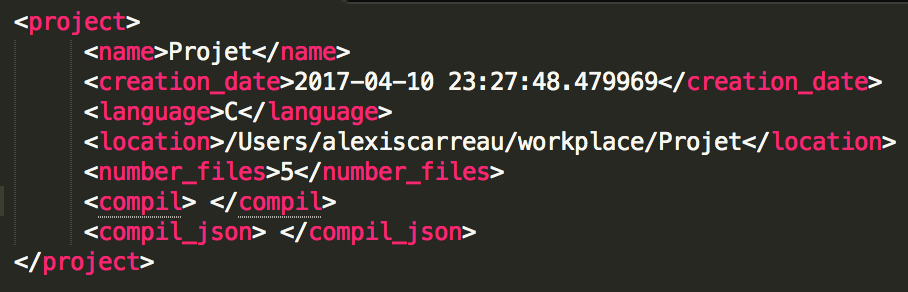
\includegraphics[scale=0.6]{images/projet_xml.png}
				\caption{Exemple de fichier xml de projet}
			\end{center}
		\end{figure}
	
\section{Conclusion}

En conclusion, nous pouvons dire que le XML est vraiment très pratique et nous l'avons utilisés dans la mesure du possible dans notre IDE pour permettre une facilité d'exécution des différentes fonctionnalités le composant. En amélioration, on pourrait imaginer la prise en compte total de tous les projets dans le fichier xml déjà alloué avec sa mise à jour lors de la suppression ou la modification des informations de projet.
		
\end{document}